\section{Protocolo de Comunicação}
\subsection{Message Queue Telemetry Transport}
	Consiste em um protocolo de mensagens leves, criado para comunicação M2M (Machine to Machine). Por exigir muito pouco processamento e banda ou consumo de internet, este é um dos protocolos ideais para dispositivos embarcados. Por esta razão, o MQTT é famoso no conceito IoT (Internet of Things).
	Uma comunicação MQTT é composta das seguintes partes: os Publishers, que irão disponibilizar as informações, os Subscribers, que são responsáveis por receber as informações e o Broker, que é o servidor MQTT acessível de qualquer lugar que possua conexão com internet.
	O funcionamento deste protocolo é simples, basicamente os publishers enviam informações para o broker, os subscribers recebem essas informações e o broker é responsável por gerenciar essa troca de informações entre eles. Este procedimento é mostrado a seguir.
    \begin{center}
    	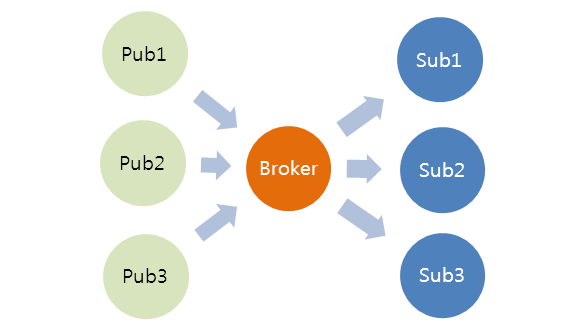
\includegraphics[scale=0.7]
        {figuras/MQTT-Funcionamento}
        \captionof{figure}{Funcionamento do protocólo MQTT}
        \label{mqtt}
    \end{center}
    
	A partir do Broker MQTT, as bibliotecas MQTT cliente podem ser utilizadas para obter os serviços de publicação e leitura dos dados do Broker. No geral a estrutura das bibliotecas contém os seguintes requisitos para conexão, publicação e inscrição:  
    \begin{itemize}
    \item 
    	Configuração do Servidor MQTT
   	\item
    	Configuração de credenciais (Usuário, senha e ID do dispositivo)
    \item
   	 	Funções de conexão
    \item
   	 	Implementação da função callback
    \item
    	Funções de inscrição e publicação.        
    \end{itemize}
    
    No geral as funções efetuam as configurações e conexões básicas para a comunicação MQTT. No entanto, a função callback merece maior atenção.
	Ao efetuar a inscrição em um tópico MQTT, o sistema cria um “gerenciador de notificações” que, em sistemas operacionais, é um thread que gerencia um socket para recebimento das mensagens de atualização no tópico inscrito. Portanto, ao detectar o recebimento de alguma atualização o sistema em thread efetua a chamada da função call-back, possibilitando o tratamento das informações provenientes da mensagem.
	Em geral a função call-back é padronizada, e tem a seguinte estrutura: 
    \textbf{callback(char* topic, byte* payload, unsigned int length);}.
    Onde: topic representa o tópico referente a mensagem recebida, payload é o conteudo da mensagem atualizada no Broker MQTT e length é o tamanho da mensagem recebida.
	É importante lembrar que todas as mensagens serão recebidas pela função callback, independentemente do número de tópicos inscritos. Para diferenciar os dados basta utilizar a variável que referencia o nome do tópico da mensagem. Portanto, com tais componentes é possível manipular dados recebidos pelas inscrições.
    
\section{Módulos de Processamento}
\subsection{Módulo WiFi ESP8266}
	O chip ESP8266 é um módulo wireless de baixo custo com 11 portas GPIO (General Purpose Input/Output) com um processador ARM. Este módulo é bastante usado para aplicações com IoT (Internet of Things) e automação.
	O ESP8266 possui uma variedade de versões, e essas versões podem ser apenas o chip ou já integrada em uma placa chamada de “Node mcu” com todas as conexões prontas para uso, bastando apenas conectar em um computador para programa-lo. A versão utilizada neste projeto foi o modelo ESP8266-12E sem o Node mcu, segue em anexo na figura.
    \begin{center}
    	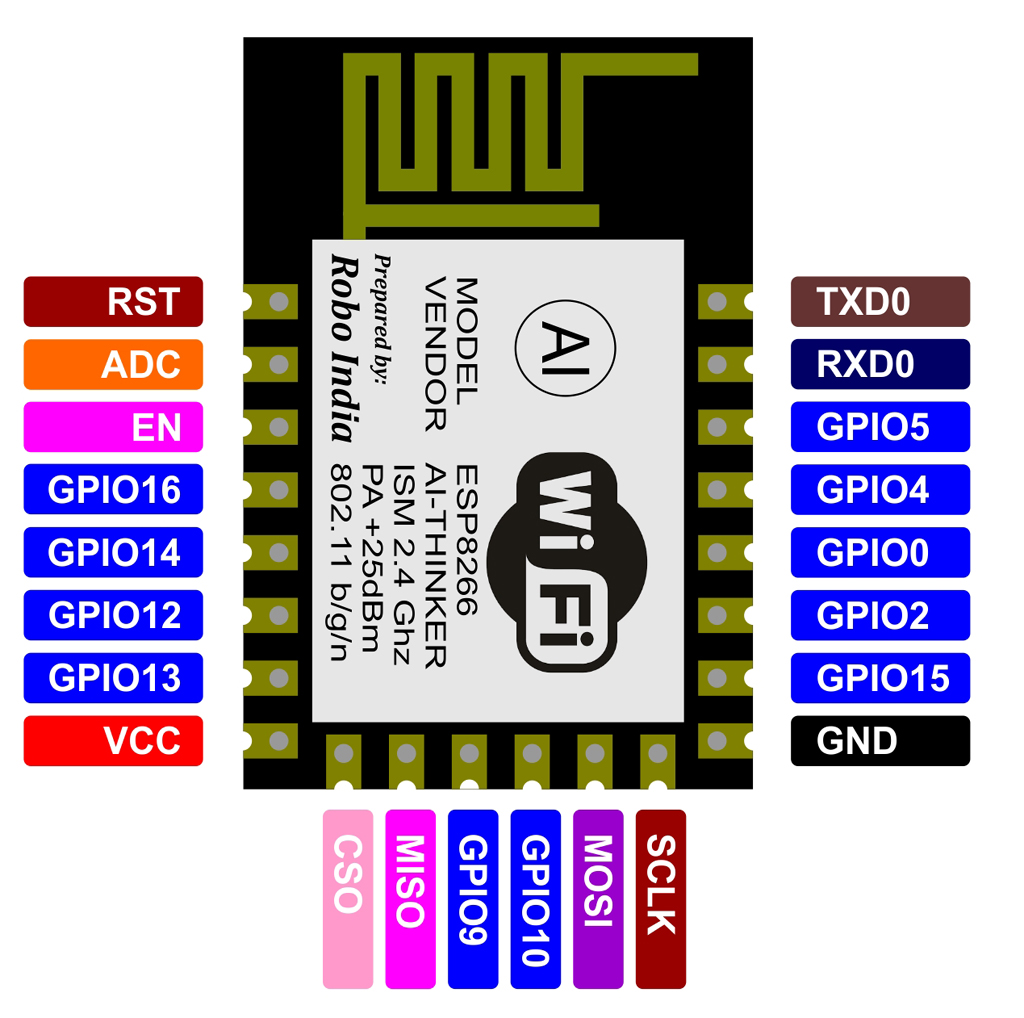
\includegraphics[scale=0.9]{figuras/esp_pinout}
        \captionof{figure}{Portas do módulo WiFi ESP8266.}
    \end{center}   
	Por ter sido usado um modelo que possui apenas o chip, todas as ligações necessárias para poder programar o módulo foram realizadas manualmente. As ligações realizadas podem ser visualizadas a seguir na figura.
    \begin{center}
    	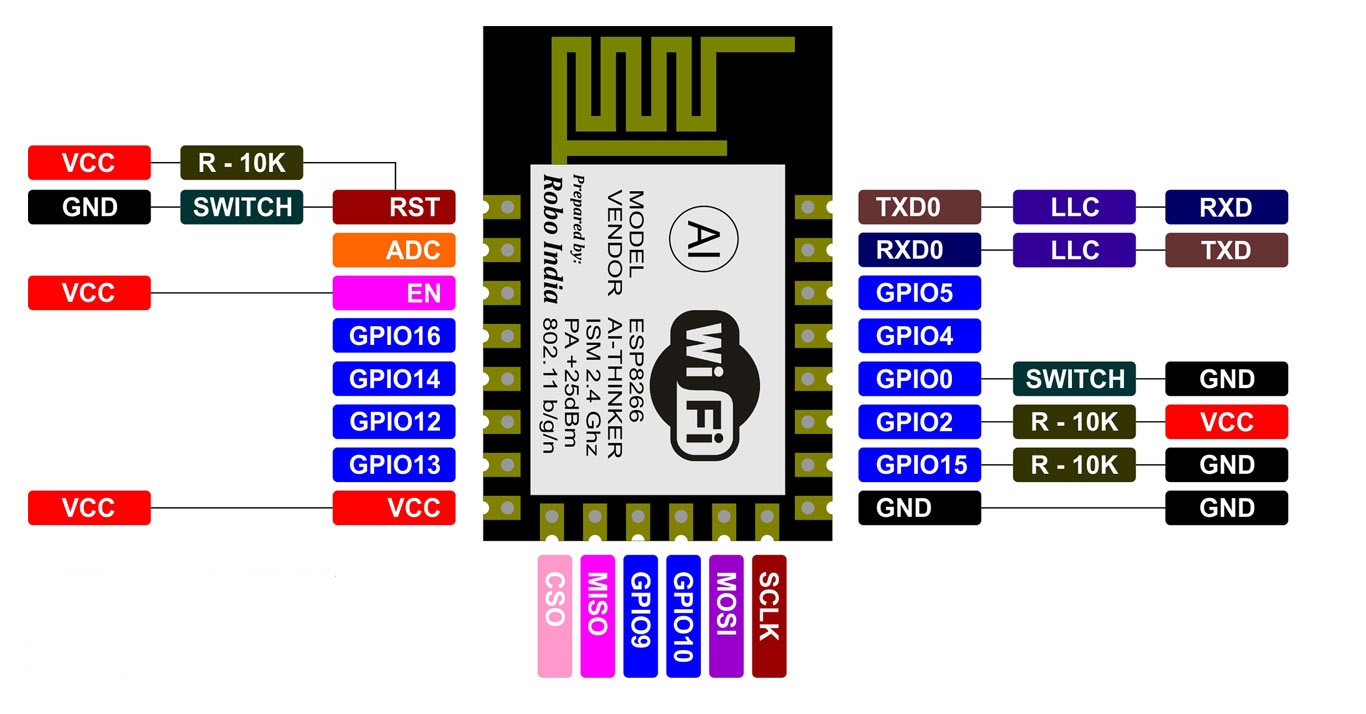
\includegraphics[scale=0.5]{figuras/esp_connects}
        \captionof{figure}{Conexões necessárias para programar o módulo ESP8266.}
    \end{center}
    Para poder programar este módulo é necessário entender os seus modos de operação. O ESP8266 possui dois modos de operações, são eles o Flash Boot e o modo UART. O modo de flash boot é basicamente o modo em que ele está pronto para receber o código que vai ser executado, já o modo UART é o modo em que o modulo vai estar em execução do código que está presente em sua memória flash. Os pinos responsáveis por alternar entre os modos de operação são os pinos de reset e GPIO0. Para manter o módulo em Flash Boot o pino GPIO0 deve estar conectado ao GND e logo após ativar e desativar o reset. E para manter em modo UART mantém-se o GPIO0 em VCC e realiza o mesmo procedimento de reset. Isso explica o uso dos “Switches” nos pinos de reset e GPIO0, utilizado unicamente para alterar os modos de operação do ESP.
	Este módulo pode ser programado utilizando a IDE do Arduino ou utilizando a interface ESplorer, que faz uso da linguagem LUA para programá-lo.

\subsubsection{Especificações do ESP8266-12E}

\begin{itemize}
\item 
	Protocolo 802.11 b/g/n
\item
	Antena embutida
\item
	Modos de operação: STA/AP/STA+AP
\item
	Suporta 5 conexões TCP/IP
\item
	GPIO com funções de PWM, I2C, SPI, etc
\item
	Taxa de transferência: 110-460800bps
\item
	Conversor AD (1V de entrada).
\end{itemize}

\subsection{Raspberry Pi 3}

O \textit{Raspberry Pi}, diferentemente de microcontroladores potencialmente utilizáveis para realizar esse projeto, permite o \textit{multitasking} do \textit{software} nele embarcado. Essa característica é importante para a coordenação de vários subsistemas necessários para solucionar o problema a que o projeto se propõe a lidar. As especificações que foram levantadas no início do projeto, a exemplo da modularização dos sensores, podiam ser atendidos com outro microcomputadores, contudo, o Raspberry possui sistemas operacionais dedicados e aplicações dos protocolos de IoT (Internet das Coisas) mais robustos. 

Especificações Raspberry Pi 3:
\begin{itemize}
\item Processador Broadcom BCM2837 64bit ARMv8 Cortex-A53 Quad-Core
\item Clock 1.2 GHz
\item Memória RAM: 1GB
\item Adaptador Wifi 802.11n integrado
\item Bluetooth 4.1 BLE integrado
\item Conector de vídeo HDM
\item 4 portas USB 2.0
\item Conector Ethernet
\item Interface para câmera (CSI)
\item Interface para display (DSI)
\item Slot para cartão microSD
\item Conector de áudio e vídeo
\item GPIO de 40 pinos
\item Dimensões: 85 x 56 x 17mm
\end{itemize}

No Raspberry foram desenvolvidas as configurações de rede. Nele foi feito um access point para que os sensores wireless pudessem se conectar ao broker. Além do mais, ele permite a utilização do cabo de rede para conexão com o computador que irá gerar os gráficos do jogo. As configurações setadas estão no Raspberry estão explicadas passo a passo no apêndice XXX.
\subsection{Conversor Analógico-Digital ADC0809}

	Para fazer a conversão analógico-digital dos dados de frenagem e posição angular do guidão foi usado o conversor analógico-digital ADC0809, devido ao Raspberry Pi 3 não possuir conversores analógico-digitais. O ADC0809 é um conversor de 8 bits de resolução e frequência de amostragem de 10 kHz. O conversor conta com 8 canais de entrada independentes e saída paralela de 8 bits. 

	O conversor conta com seis entradas de controle. Três entradas de seleção do endereço de entrada (\textit{ADD A – Address A, ADD B – Address B e ADD C – Address C}), uma entrada para atualizar o endereço do canal setado nas seletoras (\textit{ALE – Address Latch Enable}), uma entrada para habilitar a saída (\textit{OE – Output Enable}) e uma entrada para dar início a conversão (\textit{START}).

	O conversor também tem um sinal de interrupção (EOC – \textit{End of Conversion}) que indica quando a conversão iniciou e termino. O sinal quando não há conversão fica em nível alto, quando uma conversão é iniciada o sinal vai para nível baixo e quando a conversão é finalizada o sinal volta para nível alto, indicando o fim de conversão.

	Há ainda os sinais de referência do sinal de entrada que servem para condicionar o sinal de entrada para máximo aproveitamento de resolução e o sinal de \textit{clock} de clock com uma frequência de 500 kHz. Este sinal de \textit{clock} foi gerado com o LM555 em modo ástavel. 

	Para fazer uma conversão primeiro deve se definir o canal através de seu endereço usando entradas de controle seletoras, depois atualizar o endereço com a entrada de controle \textit{ALE} e setar o sinal de \textit{START}. Após isso basta esperar a interrupção \textit{EOC} acusar fim de conversão e habilitar a saída com \textit{OE} para entregar o resultado da conversão a GPIO do Raspberry Pi 3.



\section{Circuitos de Aquisição de Dados}

\subsection{Circuitos de Aquisição de Dados da Bicicleta}

\subsubsection{Sensor de RPM e velocidade}    

		Para o sistema responsável por aferir a velocidade da corrida do usuário foi usado o sensor de proximidade infravermelho ajustável E18-D80NK da Tinkbox. Este sensor de modelo comercial foi escolhido por apresentar uma estrutura cilíndrica de fácil acoplamento, sendo requisitado apenas um furo em uma superfície para prendê-lo com suas próprias roscas de fixação.
        
            \begin{center}
    	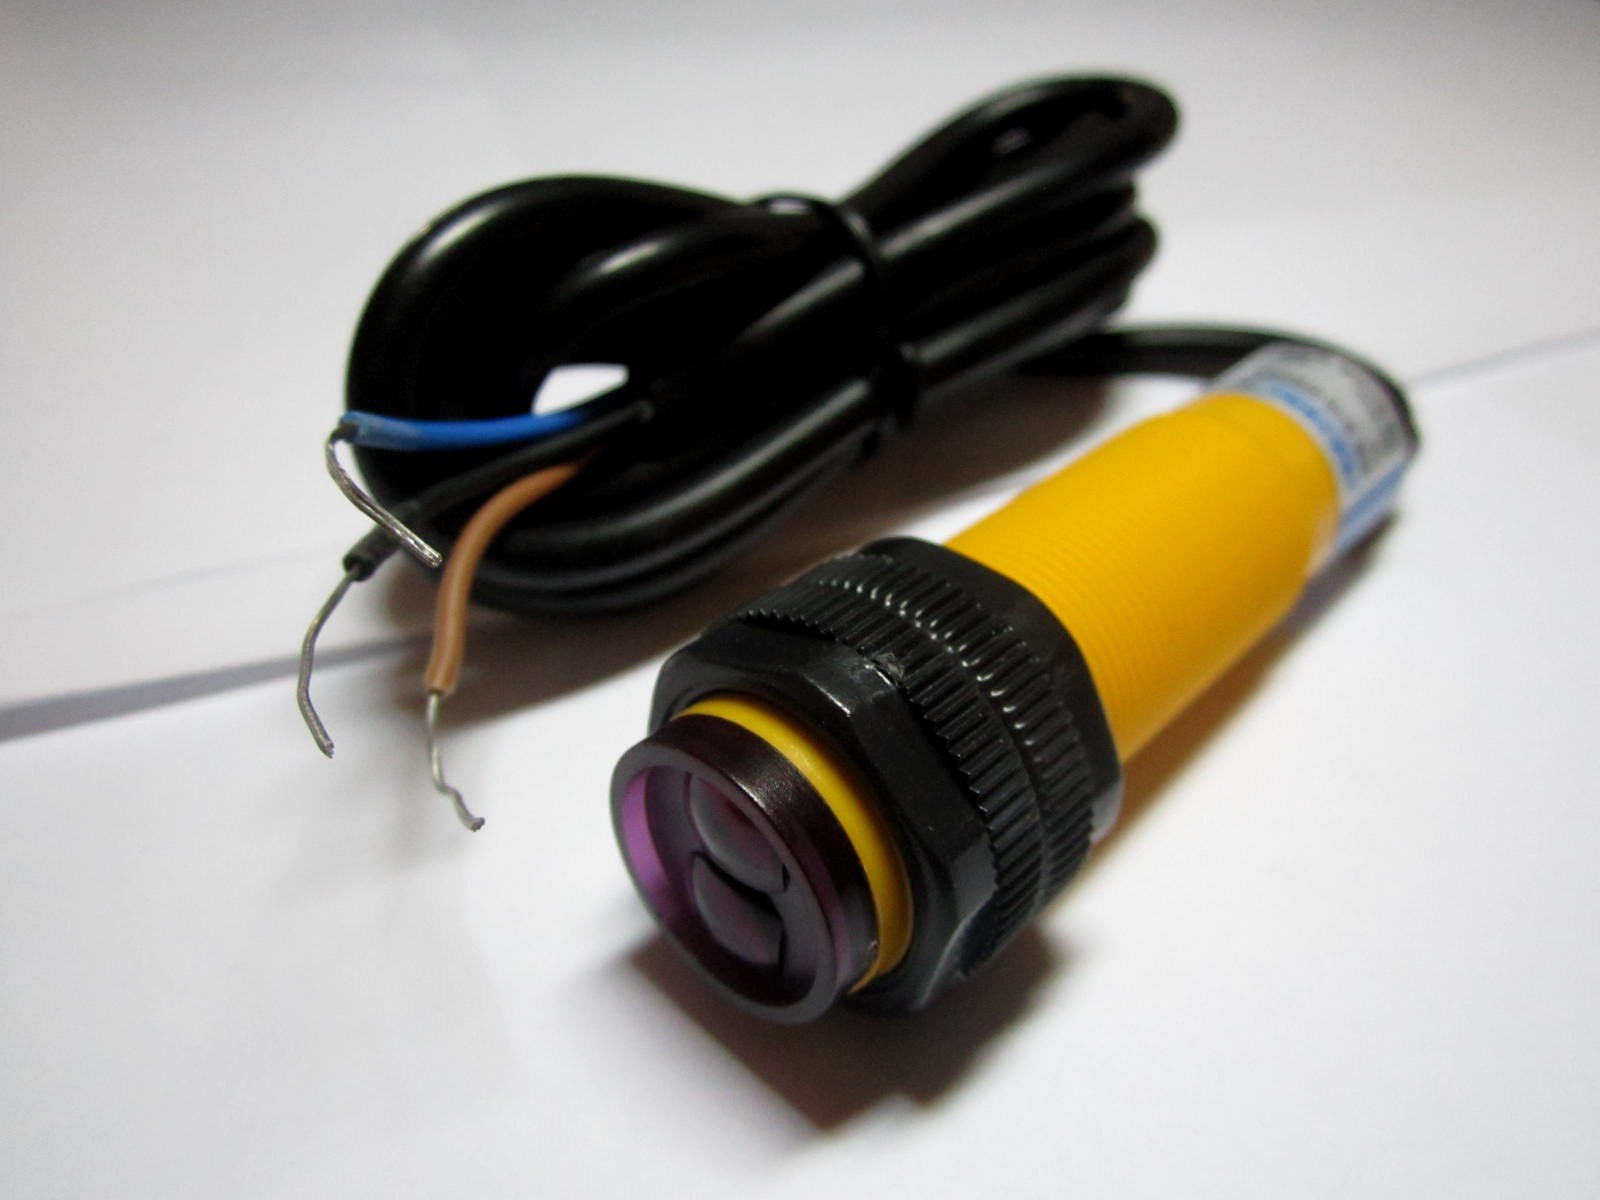
\includegraphics[scale=0.40]{figuras/ed18.jpg}
        \captionof{figure}{Sensor de proximidade infravermelho ED18-D80NK.}
        \label{ir_model}
    \end{center}
    
	O sensor é do tipo ativo e conta com um transmissor de sinal IR, um LED IR, e um receptor de sinal IR, um fototransistor. O sinal emitido pelo LED IR é refletido para o sensor com encontra algum obstáculo e é detectado pelo fototransistor TBJ NPN. A distância que é alcançada pelo sinal emitido pelo LED IR é controlada pela tensão sobre o mesmo, esta tensão é regulada por um \textit{trimpot}, sua variação faz com que o alcance do sinal IR emitido consiga refletir objetos em distâncias de 3 a 80 cm. 
    
            \begin{center}
    	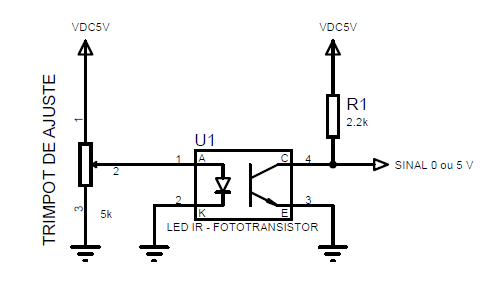
\includegraphics[scale=0.70]{figuras/IR_CIRCUIT.png}
        \captionof{figure}{Esquemático do circuito do sensor de proximidade ED18-D80NK.}
        \label{ir_circuit}
    \end{center}

	A saída do sinal é puramente digital. Enquanto o fototransistor não detecta o sinal IR refletido não há condução de corrente, logo não a queda de tensão no resistor \textit{R1} da Fig.\ref{ir_circuit} e a saída tem o valor da tensão DC de alimentação. Se o fototransistor detecta o sinal refletido este é polarizado e passa a conduzir, com isso o sinal de saída passa a ser o valor da queda de tensão sobre o fototransmissor, que pode ser interpretado com 0 pelo Raspberry Pi 3, uma vez que sua documentação acusa de tensões entre 0 e 0,8 V são interpretadas com nível baixo na entrada de sua GPIO.
    
    	Para contar a velocidade com este sensor primeiro são calculadas as rotações por minuto do rolo ao qual o rolo da bicicleta está em contato, para isso, no rolo foi conectado um nível em formato de paralelepípido com 2 cm de altura, como consta na Fig.\ref{ir_nivel}. Deste modo é possível ajudar o sensor para detectar apenas o nível a cada rotação.
        
           \begin{center}
    	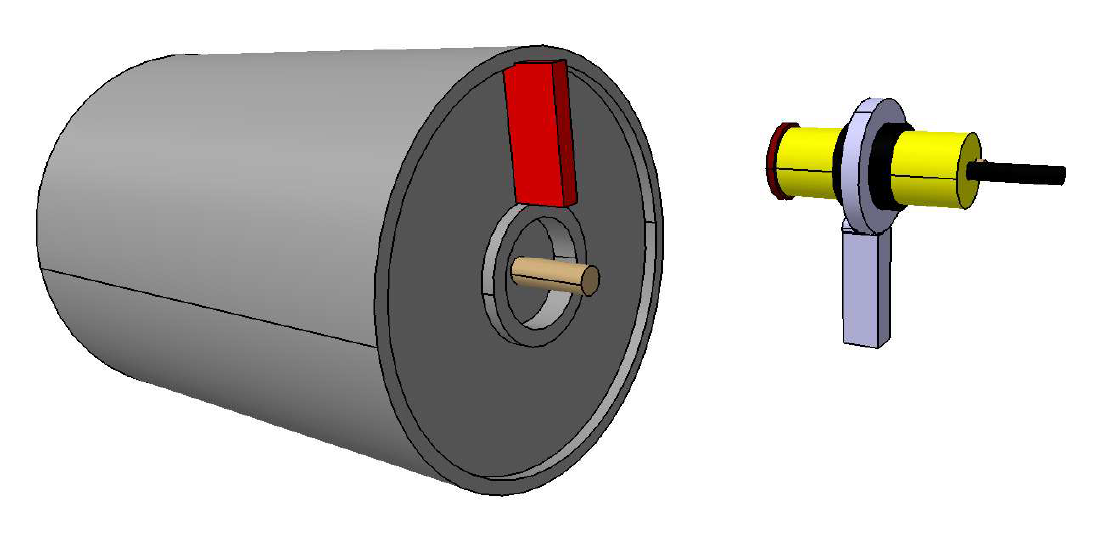
\includegraphics[scale=0.57]{figuras/ir_nivel.png}
        \captionof{figure}{Esquema de posicionamento do sensor de proximidade infravermelho para contagem de RPM.}
        \label{ir_nivel}
    \end{center}        
    
    	A saída do sensor é conectada na Raspbery Pi 3. Na Raspberry  Pi 3 foi implementado um código em python que conta as bordas de descida na porta de GPIO a qual a saída está conectada. Esta borda de descida indica que o sensor detectou uma rotação. A lógica implementada no código consiste em contar quantas rotações ocorrerão em um segundo e então multiplicar esse número por 60 para se ter um valor de RPM. Toda vez que há uma borda de descida uma interrupção é chamada e um contador é incrementado, a cada segundo é feito o cálculo em cima do valor do contador e este é zerado em seguida para se iniciar uma nova contagem.
 
    

\subsection{Circuitos de Aquisição de Dados da Fisiológicos}

\subsubsection{Atividade Eletrodermal via GSR}
No estudo dos sinais fisiológicos na Engenharia Biomédica o sinal de Atividade Eletrodermal é um dos mais importantes, isto devido ao fato de que a sua resposta é baseada nas características elétricas da pele. Sabe-se a mais de 100 anos %(referência: Vigouroux, R. (1888). The electrical resistance considered as a clinical sign. Progres Medicale, 3, 87-89.) 
que a resposta galvânica da pele é um efeito proveniente das regiões periféricas e que, muitas das vezes, pode ser utilizado como uma medida para níveis de estresse em diversas situações %(referência: https://www.researchgate.net/profile/Rebecca_Elliott2/publication/12565836_Neural_activity_relating_to_generation_and_representation_of_galvanic_skin_conductance_responses_A_functional_magnetic_resonance_imaging_study/links/00b4952dd499abb525000000.pdf). 
	Para mensurar o nível de estresse no ambiente virtual, um dos objetivos propostos pelo trabalho, utilizou-se então de um circuito GSR (Galvanic Skin Response) desenvolvido na dissertação de %(Miranda, 2014) (referência: DESENVOLVIMENTO DE BANCADA PARA SIMULAÇÃO VEICULAR INTEGRANDO REALIDADE VIRTUAL E MEDIÇÃO DE DADOS FISIOLÓGICOS,  MATEUS RODRIGUES MIRANDA) 
almejando disponibilizar para o usuário informações sobre o nível de estresse, os quais podem ser comparados a posteriori com atividades fora da realidade virtual.
	O circuito utilizado possui dois seguidores de tensão, que têm como objetivo diminuir o consumo de energia, pois o circuito é alimentado por bateria e tende-se a facilitar a manutenção para usuário final. Ainda usufrui-se de dois filtros passa-baixas, com frequências de corte teóricas de 60Hz e 120Hz (harmônicos advindos da rede de energia elétrica). Utilizou-se então dois filtros com seguidores de tensão, os quais podem ser observados no esquemático %XXX 
, realizando algumas alterações nos valores dos componentes para ser possível a utilização de componentes comerciais.
	Os resultados obtidos em simulação, podem ser observados na Fig.\ref{gsr_sim}.
    
    \begin{center}
    	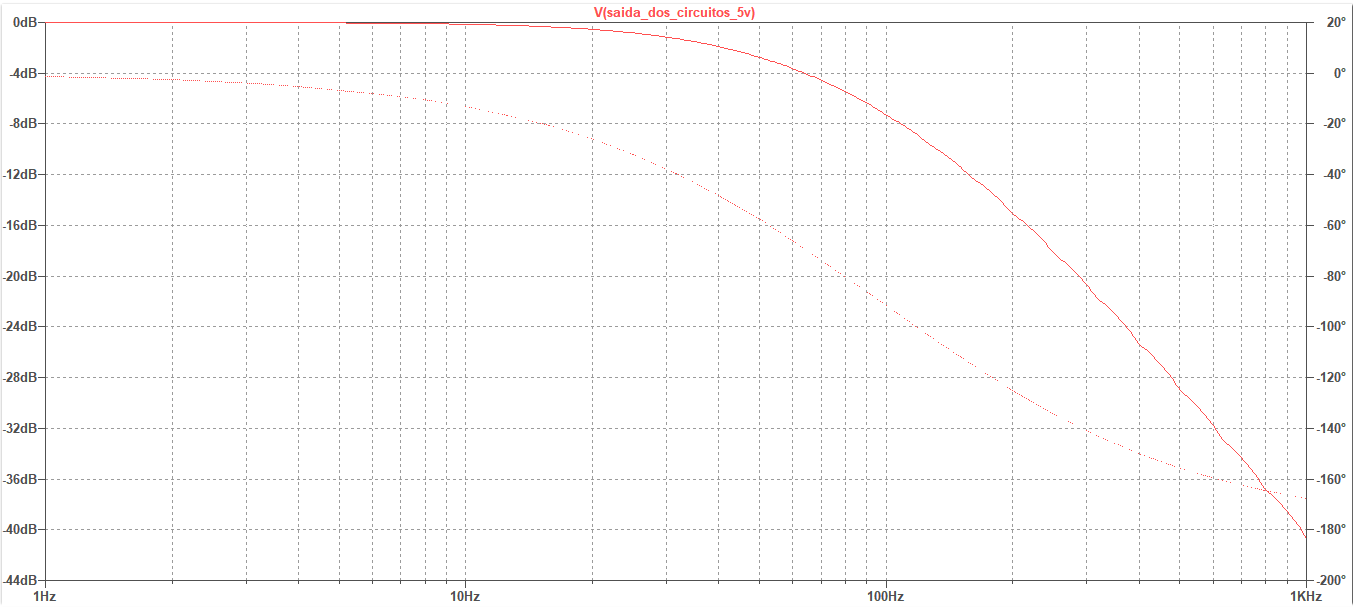
\includegraphics[scale=0.3]{figuras/Resultados_Simulacao_GSR}
        \captionof{figure}{Resultado da Simulação do GSR}
        \label{gsr_sim}
    \end{center}
    
    Foram elaborados também terminais específicos para o dedo, melhorando a superfície de contato, tendo em vista que este circuito tem que ficar em extremidades do corpo (sensibilidade do circuito simpático), ou seja, ficará próximo à mão do atleta.
    

\subsubsection{Frequência Cardíaca}

Outro sinal muito importante no diagnóstico de doenças cardiovasculares e do esforço exercitado nas atividades físicas é o sinal de frequência cardíaca. Ele ajuda os profissionais da saúde a entenderem melhor os efeitos de doenças como: miocardiopatia, hipertensão arterial, epilepsia, entre outros. %(referência: http://www.scielo.br/scielo.php?pid=S0102-76382009000200018&script=sci_arttext&tlng=pt) . 
	O usuário da plataforma Vride terá disponível este sinal para avaliação do seu rendimento e comportamento na atividade física desenvolvida dentro do ambiente. Estes dados podem ser usufruidos para análise de profissionais da educação física ou da medicina para detectar o parâmetros importantes na elaboração de treinamentos ou tratamentos destas doenças. 
	
    Na literatura disponível, possuem diversas topologias para adquirir este sinal de frequência cardíaca, contudo, a ideia é ter um método não invasivo com a maior precisão possível. Então, após um refinamento dos artigos pesquisados, foi definido que a técnica de fotopletismografica atendia aos nossos critérios de custo e precisão, e foi encontrado um artigo em que era tal plataforma era desenvolvida por %(referência: Photoplethysmography (PPG) system, Geert Langereis)
    , mas algumas características de filtragem foram extraídas por foram retiradas de %(referência: Non-Invasive Measurement of Heart Rate and Hemoglobin Concentration Level Through Fingertip) (referência: DESIGN AND ANALYSIS OF ARTIFACT-RESISTIVE FINGER PHOTOPLETHYSMOGRAPHIC SENSORS FOR VITAL SIGNMONITORING) . 
	
    O circuito desenvolvido utiliza de um sensor optoeletrônico de refletância, composto de um LED (diodo emissor de luz) e um fototransistor. Segundo a topologia escolhida, devem-se haver dois estágios de filtragem. Portanto, seguindo o design apresentado na Fig. %XXX
    , foram feitos circuitos para amplificação de 65 dB, tendo em vista que o sinal possui uma amplitude muito baixa, filtrado na faixa de 1Hz a 5Hz. Pôde-se observar então nas simulações:
    
    \begin{center}
    	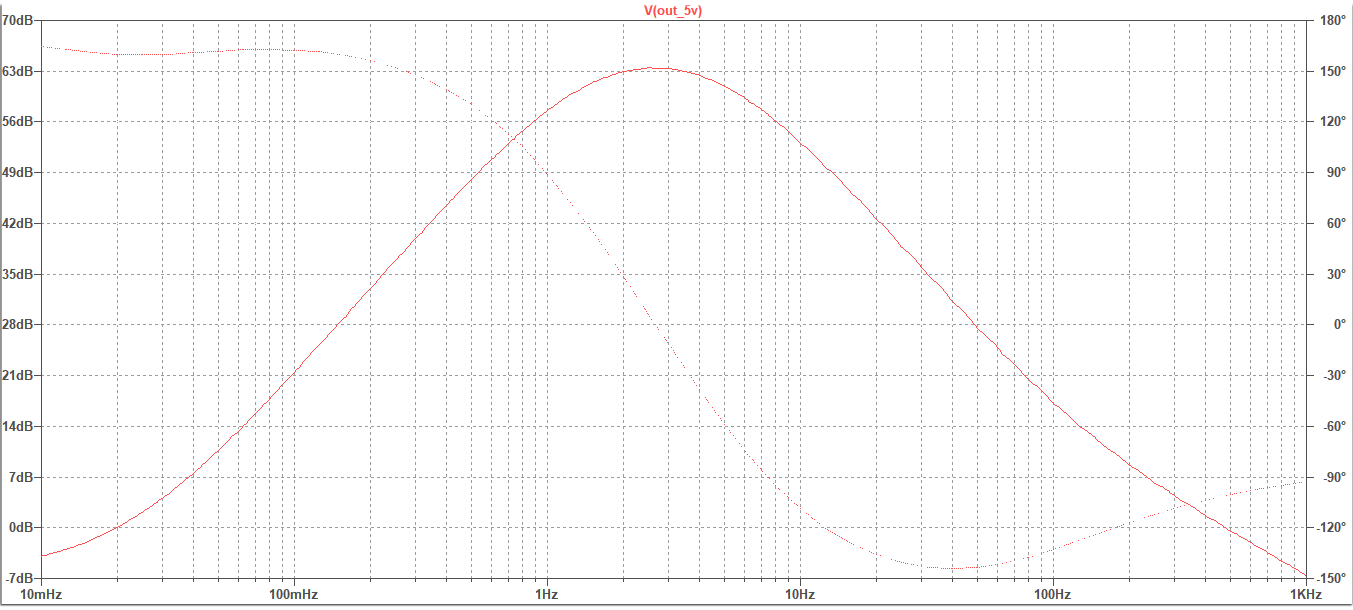
\includegraphics[scale=0.3]{figuras/Simulacao_Cardio}
        \captionof{figure}{Resultado da Simulação do Circuito de Frequência Cardíaca}
        \label{cardio_sim}
    \end{center}
    
\subsubsection{Estimação de Frequência Respiratória com Uso de FSR}

	Um dos dados fisiológicos que presta informação útil acerca do estresse causado pela atividade de ciclismo é a frequência respiratória. Esta grandeza varia proporcionalmente a frequência cardíaca, uma vez que com o aumento da frequência cardíaca mais sangue é enviado aos pulmões e logo há uma maior demanda de taxa trocas de gasosas [1].  Monitorar esse dado ajuda a perceber se o usuário está respirando de maneira correta para o melhor desempenho.
    
	Para se mensurar a frequência respiratória efetivamente deve se aferir as trocas gasosas em cada respiração, esta demanda exige que um aparato seja conectado ao redor das vias nasais para fazer a medida [2]. Para o escopo do trabalho esta medida não pode ser implementada visto que o usuário já estará usando um óculos de realidade virtual consideravelmente grande e este aparato traria um incomodo para o usuário, o que provavelmente o faria não usar a solução ou interferir na análise de estresse causada.
    
	Uma solução para suprir essa demanda é ao invés de aferir as trocas gasosas aferir a expansão da caixa torácica a cada respiração do usuário. Quando o usuário respira a variação de gás no pulmão faz com este se contraia e expanda, ao se ler o nível dessa expansão é possível ter uma boa estimativa da frequência respiratória do atleta [2].
    
	Para e verificar a expansão da caixa torácica foi usado um FSR (Force-Sensing Resistor) este dispositivo é um material que tem sua resistência elétrica variada de forma inversamente proporcional a tensão mecânica aplicada em sua superfície. Logo, basta colocar um FSR com sua superfície em contato com o tórax do atleta.
    
    \begin{center}
    	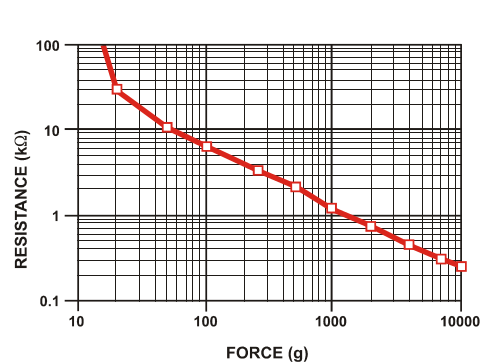
\includegraphics[scale=0.5]{figuras/fsr_resistance_force.png}
        \captionof{figure}{Curva típica de um FSR.}
        \label{fsr_curve}
    \end{center}

	O FSR usado foi o de modelo quadrado de lado medindo 4,38 cm da Interlink Electronics. Sua resistência varia de um valor de mais de 1MOhm, quando está sem carga, para algumas unidades de Ohm, quando está saturado de carga [3].
    
    \begin{center}
    	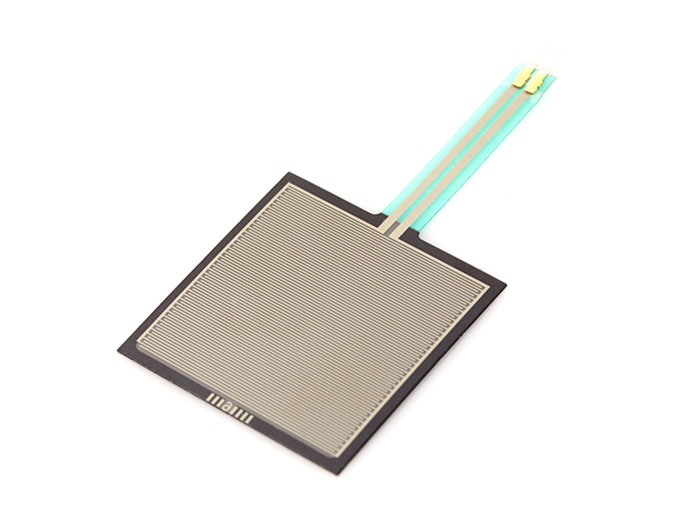
\includegraphics[scale=0.4]{figuras/fsr_model.jpg}
        \captionof{figure}{Modelo de FSR usado.}
        \label{fsr_model}
    \end{center}

	Como componente elétrico o FSR pode ser tratado com uma resistência variável. Logo, é possível associá-lo com outros resistores e aferir a tensão do divisor de tensão gerado. Esta tensão irá variar de acordo com a variação do FSR. Deste modo, o FSR foi colocado como resistência variável em uma topologia de ponte de Wheatstone desequilibrada.
    
	O circuito montado para o estimador de respiração usado está no Anexo I, a saída da ponte de Wheatstone é conectada um amplificador diferencial DC de alta impedância de entrada, a topologia do amplificador diferencial usa dois estágios de amplificadores LM324 e foi baseada em um esquemático que consta no próprio datasheet do mesmo. O LM324 foi escolhido devido a não precisar de alimentação simétrica, podendo ser alimentado apenas com 5 V. 
    
	Após o estágio diferenciador o sinal é passado através de um filtro RC Passa-Baixas de 1ª ordem, com frequência de corte de 34 Hz. Um adulto possuí uma frequência de movimentos respiratórios por minuto entre 12 e 48 movimentos [4], logo uma frequência baixa ade 34 Hz é suficiente para preservar o sinal de variação lenta. Após o estágio de filtragem o sinal é passando por um \textit{buffer} e um divisor de tensão para condicionar o sinal de saída para próximo de 1 V, valor de entrada do conversor analógico-digital do módulo transmissor ESP2866.
    
    O circuito do estimador de respiração foi simulado no software ADS 2009, da Agilent. A figura de sua simulação consta na Fig.\ref{fsr_ads}.  
    
    
    \begin{center}
    	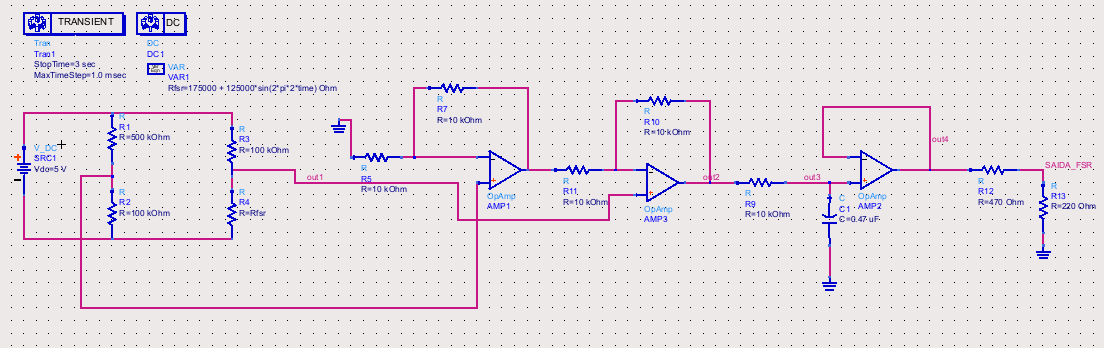
\includegraphics[scale=0.42]{figuras/fsr_ads.png}
        \captionof{figure}{Simulação do estimador de respiração no software ADS.}
        \label{fsr_ads}
    \end{center}
    
 	Para validar o circuito foram feitas duas simulações uma simulação paramétrica e uma transiente. Na simulação paramétrica foi variado a resistência que representa o FSR de 1 $\Omega$ a 1 M$\Omega$ para ver o comportamento do circuito dentro dos limites possíveis da variação do FSR. Este resultado consta na Fig.\ref{fsr_param}. Na figura, os dois \textit{markers} indicam os valores de resistência de 50 k$\Omega$ e 300 k$\Omega$, através de testes com o FSR em contato com a caixa torácica percebeu que a expansão e contração da mesma tende a manter o valor de resistência do FSR entre estes valores. Deste modo o circuito foi condicionado para que este \textit{range} de valores esteja bem alocado no valor de 0 a 1 V de tensão de saída.
    
    
        \begin{center}
    	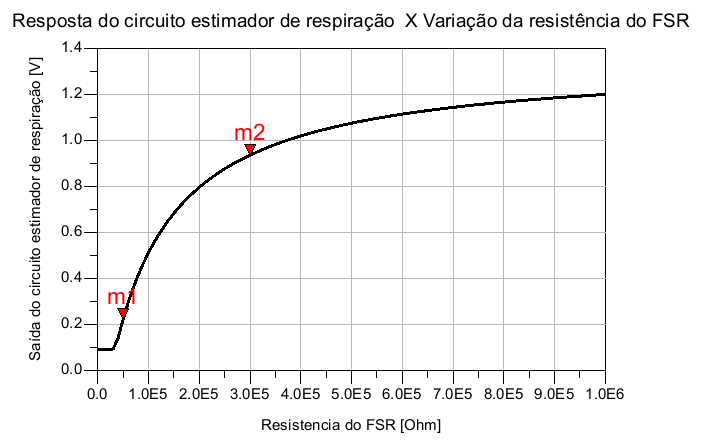
\includegraphics[scale=0.5]{figuras/SaidaFSR_X_resFSR.png}
        \captionof{figure}{Resultado da simulação parâmetrica do estimador de respiração no software ADS.}
        \label{fsr_param}
    \end{center}
    
    Para a simulação transiente foi atribuida uma função para a resistência do FSR apresentada na Eq.\ref{eq1}. Essa função emula a resistência do FSR quando em contato com a caixa toráxica para um ritmo extremo de duas respirações por  segundo. Para sua modelagem foram considerados os limites de excursão frequentes da resitência do FSR quando em contato com a pele. Quando a função seno está em seu máximo a resistência tem 300 k$\Omega$ e em seu mínimo um valor de 50 k$\Omega$. A simulação foi executada durante 3 segundos. Pode se perceber que a saída ficou no \textit{range} de saída entre 0 e 1 V.
    
\begin{equation}\label{eq1}
Resitência FSR = 175000 + 125000 \cdot \sin (2 \cdot \pi \cdot 2 \cdot t) \space \Omega
\end{equation}

    
    
            \begin{center}
    	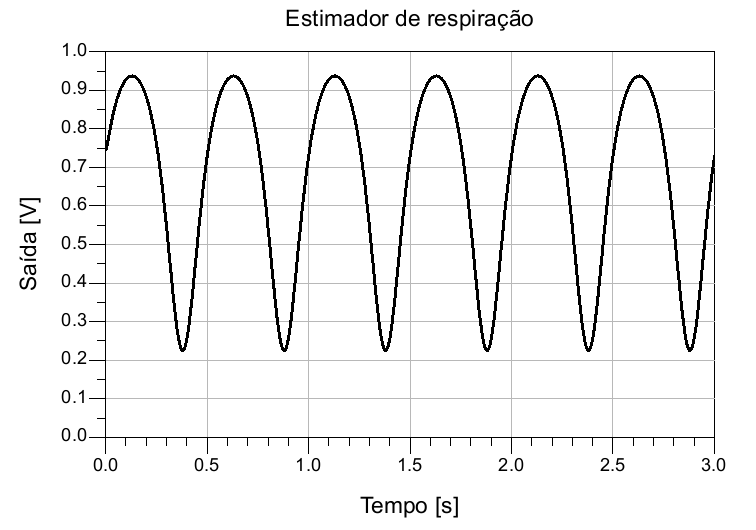
\includegraphics[scale=0.40]{figuras/transiente_FSR.png}
        \captionof{figure}{Resultado da simulação transiente do estimador de respiração no software ADS.}
        \label{fsr_tran}
    \end{center}
    
	A saída é convertida com o conversor analógico-digital do ESP8266-12E e transmitida via WI-FI até o \textit{broker} do protocolo do MQTT implementado no Raspberry Pi 3.
    O \textit{layout} do circuito foi desenvolvido no software Proteus e segue nos Anexos II. O placa desenvolvida foi de camada simples com uso de componentes PTH. Para a transferência do \textit{layout} para o cobre foi usado o processo de transferência térmica e corrosão por percloreto de ferro.
    

    
    
    
    
    
%[1] ROSERO, Oscar F. G. Sistema móvel de monitoramento e treinamento para ciclista com smartphone android. Departamento de Engenharia Elétrica, Faculdade de Tecnologia – Universidade de Brasília. FEV, 2012.


%[2] MIRANDA, Mateus R. Desenvolvimento de uma bancada para simulação veicular integrando realidade virtual e medição de dados fisiológicos. Departamento de Engenharia Mecânica, Faculdade de Tecnologia – Universidade de Brasília. DEZ, 2014.

%[3] FORCE Sensing Resistor Integration Guide and Evaluation Parts Catalog. Camarillo: Interlink Electronics. 25p.
%[4] SINAIS vitais. Paraná: SIATE – Serviço Integrado de Atendimento ao Trauma em Emergência. 2015. 26p. 



